\section{Method}
\label{sec:method}

\begin{figure*}[!t]
    \centering
    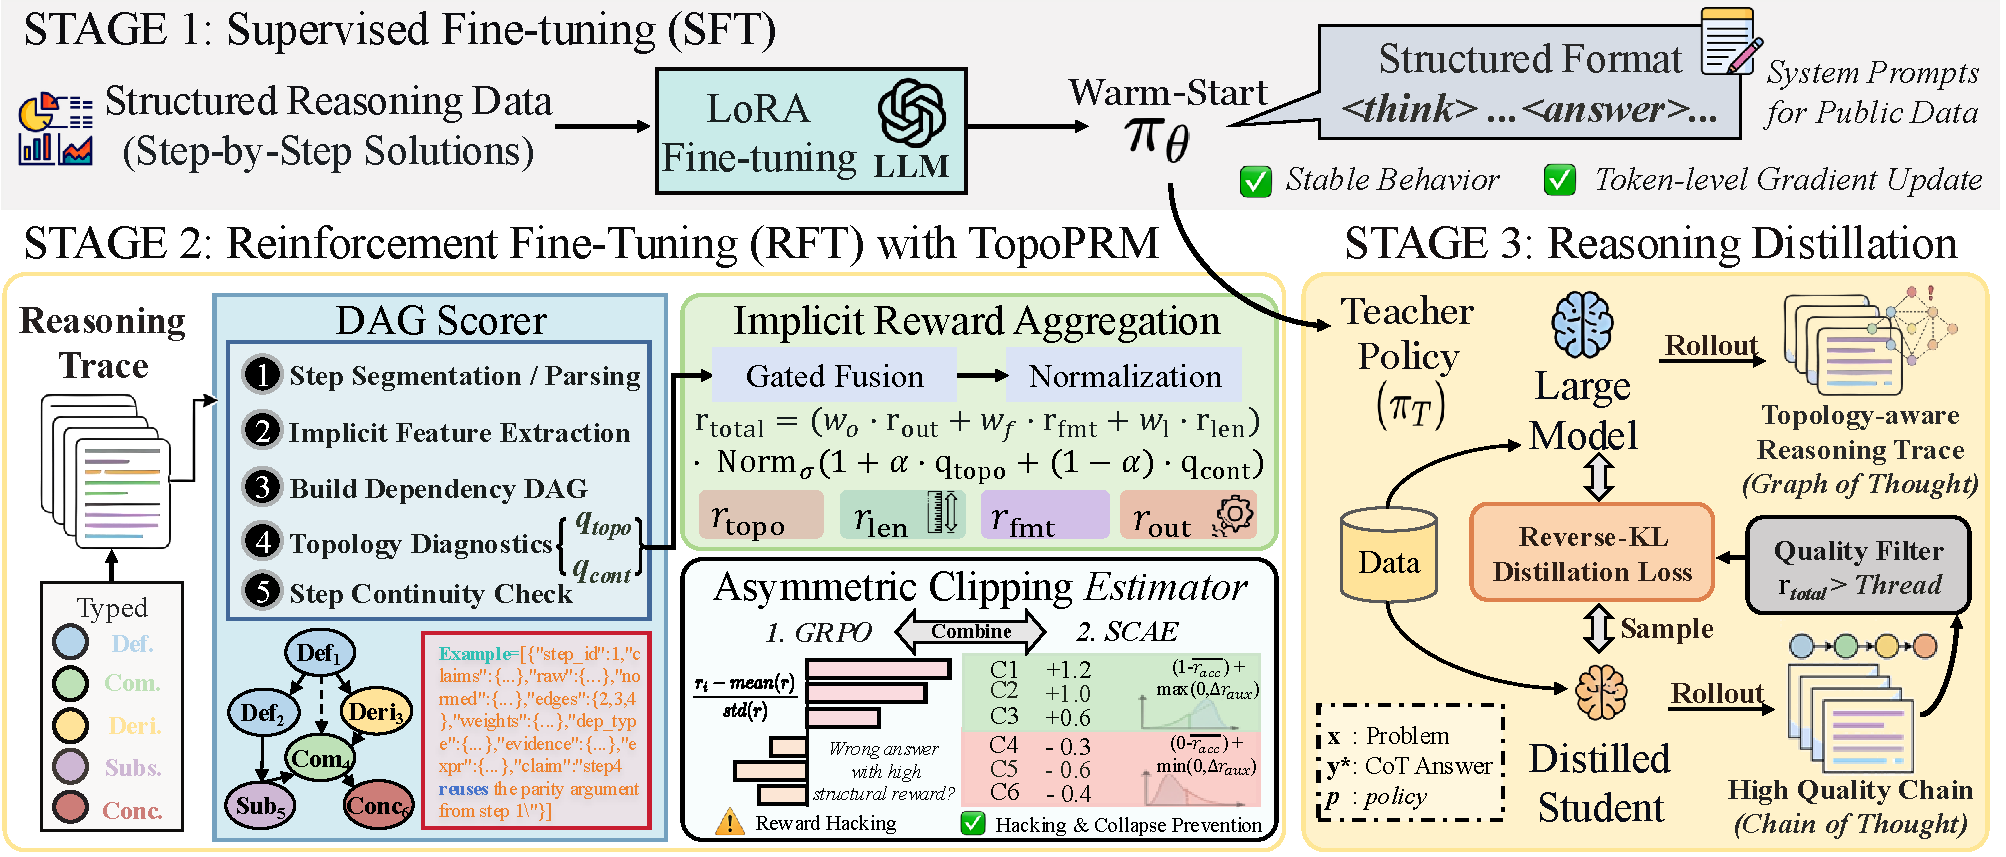
\includegraphics[width=0.98\linewidth]{figures/fig2_topoprm_framework.pdf}
    \caption{Overview of our proposed \method with its three-stage framework \framework. The deterministic DAG Scorer lifts reasoning traces into structural representations. Hierarchical multiplicative reward and asymmetric advantage clipping bound within-stratum credit. And a topology-conditioned on-policy distillation stage that compresses the long-CoT teacher into a compact student.}
    \label{fig:overview}
\end{figure*}

\framework (illustrated in Figure~\ref{fig:overview}) is a topology-aware post-training framework whose three stages are linked by a single starting point: a deterministic \textbf{DAG Scorer $\mathcal{E}$} that converts long-chain reasoning traces into a structure-sensitive form on which all downstream supervision is computed.
% \framework（图~\ref{fig:overview}）是一个以拓扑结构为感知核心的后训练框架，其三阶段共享同一起点：确定性的 DAG Scorer $\mathcal{E}$，将长链推理轨迹转化为结构敏感的表示形式，所有下游监督均在此之上计算。
Stage~I performs supervised cold start to enforce parsable formatting; Stage~II runs GRPO with the hierarchical reward that fused \textbf{TopoPRM} and Stratified Clipping Advantage Estimation (\estimation); Stage~III executes Topology-Guided Self-Distillation, in which the Stage-II teacher provides token-level reverse-KL supervision while the student rolls out under topology-conditioned revision prompts.
% Stage I 通过监督冷启动确保格式可解析；Stage II 在分层 \prm 奖励与分层裁剪优势估计（\estimation）下运行 GRPO；Stage III 执行拓扑引导的自蒸馏：Stage II 的教师以 token 级反向 KL 提供监督，而学生在拓扑条件化的修订提示下进行 on-policy 采样。
% Sharing $\mathcal{E}$ across stages turns structural supervision into a single, auditable interface, so reward shaping, advantage estimation, and trace compression all consume the same dependency graph rather than separate heuristics.
% 三阶段共享 $\mathcal{E}$ 使结构监督成为统一、可审计的接口，奖励塑形、优势估计与轨迹压缩共享同一依赖图，而非各自维护启发式规则。

\subsection{Problem Setup}
Let $x=(q,c)$ denote an input pairing a mathematical problem $q$ with optional context $c$, and let $\pi_\theta$ be a policy that generates a reasoning trace $y=(s_1,\dots,s_T)\sim\pi_\theta(\cdot\!\mid\!x)$, where each $s_i$ is a textual reasoning step. Outcome-only RLVR supervises $y$ with a sparse final-answer reward $r_{\mathrm{out}}(x,y)\!\in\![0,1]$.
% 设 $x=(q,c)$ 表示由数学问题 $q$ 与可选上下文 $c$ 构成的输入，$\pi_\theta$ 为生成推理轨迹 $y=(s_1,\dots,s_T)\sim\pi_\theta(\cdot\!\mid\!x)$ 的策略，其中每个 $s_i$ 是一段文本推理步。仅结果导向的 RLVR 通过稀疏的最终答案奖励 $r_{\mathrm{out}}(x,y)\!\in\![0,1]$ 监督 $y$。
We define $\mathcal{G}_y=(\mathcal{V},\mathcal{E}_d)$ for a directed dependency graph on $y$, with node set $\mathcal{V}=\{s_1,\dots,s_T\}$ and edge set $\mathcal{E}_d\subseteq\mathcal{V}\!\times\!\mathcal{V}$ encoding surface-evidenced support relations between steps, and $\mathcal{E}:y\!\mapsto\!\mathcal{G}_y$ for the deterministic DAG Scorer that produces it. %Throughout, $G$, $\tau$, $\alpha$, and $\widehat{A}^{(i)}$ denote the GRPO group size, the correctness threshold, the topology--continuity balance, and the per-completion advantage, respectively.
% 我们以 $\mathcal{G}_y=(\mathcal{V},\mathcal{E}_d)$ 表示在 $y$ 上构建的有向依赖图，节点集 $\mathcal{V}=\{s_1,\dots,s_T\}$，边集 $\mathcal{E}_d\subseteq\mathcal{V}\!\times\!\mathcal{V}$ 编码步间由表面证据支持的依赖关系；$\mathcal{E}:y\!\mapsto\!\mathcal{G}_y$ 为生成 $\mathcal{G}_y$ 的确定性 DAG Scorer。
\textit{Our objective is to recover latent dependency structure from $\mathcal{G}_y$ as unified supervision across SFT, RL, and distillation without human step labels or learned verifier models.
}

\subsection{Topology-Aware Data Processing}
\label{sec:reward_module}

% A central design choice of \method is to derive process-level supervision from a deterministic structural view of $y$ rather than from a learned verifier. Compared with neural PRMs, which inherit annotation noise and are vulnerable to adversarial surface forms, a rule-based extractor produces identical graphs for identical traces, so every structural reward remains reproducible and auditable on any rollout. We therefore split this stage into a graph extraction step ($\mathcal{E}$) and two normalised diagnostics ($q_{\mathrm{topo}},q_{\mathrm{cont}}$) that together form the \prm signal consumed by the hierarchical reward in \S\ref{sec:post_training}. 这一段不需要了，直接从DAG Scorer的生成和信息提取打分。然后铺垫下一段的奖励层次化聚合
% \method 的核心设计选择是从 $y$ 的确定性结构视图（而非学习式验证器）中导出过程级监督。相比继承标注噪声且易受对抗性表面形式干扰的神经 PRM，规则式抽取器对同一轨迹给出唯一的图，因此每一项结构性奖励都可在任意 rollout 上复现并被审计。本阶段相应拆分为图抽取步骤（$\mathcal{E}$）与两个归一化诊断（$q_{\mathrm{topo}},q_{\mathrm{cont}}$），共同构成 \S\ref{sec:post_training} 分层奖励所消费的 \prm 信号。

\paragraph{Trace-to-DAG Extraction}
Given $y=(s_1,\dots,s_T)$, $\mathcal{E}$ executes four deterministic stages: step segmentation by numbered markers, mathematical discourse markers, and line boundaries; sub-question partitioning that forbids cross-component edges; per-step extraction of expressions, claims, and variables; and edge construction. For ordered pair $(s_i,s_j)$ with step $i<j$ in the same sub-question, $\mathcal{E}$ inserts an implicit edge $i\!\to\!j$ when expression reuse, canonicalised claim-key overlap, or variable reference holds, after information-density filters discard single symbols, pure numerals, and heading fragments.
% 给定 $y=(s_1,\dots,s_T)$，$\mathcal{E}$ 依次执行四个确定性阶段：基于编号标志、数学话语标志（如 "$\therefore$"）与行边界的步骤切分；禁止跨连通分量加边的子问题划分；每步对表达式、claim 与变量的抽取；以及边构造。对同一子问题内每个有序对 $(s_i,s_j)$（$i<j$），当表达式复用、规范化 claim 键重叠或变量引用之一成立时，$\mathcal{E}$ 加入一条 $i\!\to\!j$ 的\emph{强}边；信息密度过滤器先剔除单符号、纯数字与标题片段。
If $s_j$ is a derivation or conclusion step lacking strong incoming support, an \emph{adaptive sequential weak} edge is added from $s_{j-1}$ only when neither $s_j$ already has strong support nor $s_{j-1}$ already emits strong outgoing dependencies, which prevents chain-dominant artefacts in long traces. Full extraction rules are deferred to Appendix~\ref{app:dag}.
% 若 $s_j$ 是缺乏强入边的派生/结论步，则仅当 $s_j$ 本身尚无强支撑且 $s_{j-1}$ 也未发出强出向依赖时，从 $s_{j-1}$ 加入一条权重为 $0.3$ 的\emph{自适应序列弱}边，以避免长轨迹中的链状伪结构。完整规则见附录~\ref{app:dag}。

% Given a reasoning trace \(y=(s_1,\ldots,s_T)\), we construct a directed graph \(G_y=(V,E)\) with one node per reasoning step. Edges are added when a later step exhibits surface evidence of depending on an earlier step. The extractor uses four types of evidence: mathematical expression reuse, normalized claim overlap, variable reference, and explicit step citation. When no strong evidence is available for a derivation or conclusion step, the extractor may add a weak sequential fallback edge for connectivity analysis, but such edges are assigned lower confidence and are not treated as proof-level support.

% The resulting graph is a structural proxy rather than a semantic proof object. Its purpose is to expose whether the trace makes its dependencies recoverable: whether conclusions have incoming support, whether edges point from premises to consequences, whether the graph remains acyclic, and whether local transitions can be traced to prior information. Full extraction rules are provided in Appendix~\ref{app:dag}.

% For a trace $y=(s_1,\ldots,s_T)$, we apply a deterministic extractor
% $\mathcal{G}=\mathcal{E}(y)=(\mathcal{V},\mathcal{A})$, where each node is a reasoning step and each directed edge denotes rule-based dependency evidence (expression reuse, claim reference, or structural connector).
% The extractor performs step segmentation, claim normalization, and edge construction with explicit fallbacks for unsupported derivation steps.
% To reduce parser artifacts, claim extraction uses sentence-level units and filters incomplete heading-like fragments before matching.

% 下面两段感觉需要凝练一下，不需要额外画一段去讲G_y的角色或者两种的得分诊断，前面我们提到了怎么建图，剩下一段我觉得应该是把1. Step Segmentation&Parsing; 2.Implicit Feature Extraction; 3.Build Dependency DAG; 4.Topology Diagnostics; 5. Step Continuity Check这几个步骤的信息没有讲清楚的给补一下，最后r_topo是怎么计算得到的。

% The graph $\mathcal{G}_y$ is a structural proxy, not a semantic proof object: it encodes whether dependencies are recoverable from the trace, not whether each step is logically valid. Determinism plays the role that proof-checking would play in a formal pipeline---identical traces yield identical graphs, training-time and test-time diagnostics share one mechanism, and structural credit can be inspected token by token without invoking a separate model. 
% $\mathcal{G}_y$ 是结构代理而非语义证明对象：它编码的是依赖是否可从轨迹中复原，而不是每一步是否逻辑成立。确定性扮演了形式化流水线中证明检查的角色——同一轨迹产生唯一图，训练与推理诊断共享同一机制，结构性信用可在不调用任何额外模型的前提下逐 token 审计。

% \subsubsection{Topology and Continuity Diagnostics}
% The two diagnostics are designed to cover complementary failure modes. The global topology score targets defects visible only at graph level---empty traces, cycles, orphan conclusions, mis-directed edges, and (when available) misalignment with a reference structure---while the local continuity score targets steps that silently introduce expressions or claims absent from the prefix.
% 两个诊断针对互补的失败模式。全局拓扑分数针对仅在图层面可见的缺陷——空轨迹、环路、孤立结论、方向错误以及（可得时）与参考结构的失配；局部连续性分数则针对悄悄引入了前缀中未出现的表达式或 claim 的步骤。

% From $\mathcal{G}$ we compute two reward-facing structural signals:
% global topology quality $q_{\mathrm{topo}}\in[0,1]$ and local continuity quality $q_{\mathrm{cont}}\in[0,1]$.
% $q_{\mathrm{topo}}$ summarizes acyclicity, orphan-conclusion support, direction consistency, and optional reference-edge alignment, capturing \emph{latent conditional dependencies} surfaced by expression and claim reuse.
% $q_{\mathrm{cont}}$ measures step-level support traceability along the weak sequential edges, capturing \emph{ordered continuity} that outcome-only supervision leaves unobserved.
% Both are produced by the same deterministic pipeline, so they act as a \emph{topology-sensitive \prm}: step-level signals that require neither human annotations nor a learned verifier, and remain fully auditable on any rolled-out trace. We treat this \prm as a structural sub-component of \method, on top of which the hierarchical reward in \S\ref{sec:post_training} is built.
% We report full definitions and term-level equations in Appendix~\ref{app:math_details}.

%\subsubsection{Scope of Verifiability}
% See Appendix for extended discussion on reward aggregation strategies.
% Our use of ``verifiable'' is operational: once a trace is produced, all reward values are computed by deterministic procedures and are therefore reproducible and auditable.
% This is distinct from semantic proof verification; we do not claim step-correctness guarantees or logical completeness.

Let $\rho_{\mathrm{orph}}(\mathcal{G})$ denote the fraction of conclusion nodes without incoming edges, $\delta(\mathcal{G})\!\in\![0,1]$ the dependency-direction consistency (premise before consequence), and $\kappa(\mathcal{G},\mathcal{G}^{\star})\!\in\![0,1]$ an optional reference alignment that activates only when a reference DAG $\mathcal{G}^{\star}$ is available. The global topology score is then
\begin{equation}
\label{eq:qtopo}
\small
\begin{aligned}
q_{\mathrm{topo}}(\mathcal{G})=\;
& \lambda_b\,\mathbb{1}[|\mathcal{V}|>0]
+\lambda_a\,\mathbb{1}[\mathcal{G}\text{ acyclic}] \\
+\lambda_o\,\mathbb{1}&[\rho_{\mathrm{orph}}(\mathcal{G})\!=\!0]
+\lambda_d\,\delta(\mathcal{G})
+\lambda_k\,\kappa(\mathcal{G},\mathcal{G}^{\star}),
\end{aligned} %这条公式太多的系数了，会让审稿人觉得不可控、缺乏验证等问题，有没有方法可以精简和优化到可验证、可学习收敛的表达。
\end{equation}
with $\lambda_b,\lambda_a,\lambda_o,\lambda_d,\lambda_k\!\ge\!0$ and $\sum_\bullet\lambda_\bullet\!=\!1$, so $q_{\mathrm{topo}}\!\in\![0,1]$.
% 设 $\rho_{\mathrm{orph}}(\mathcal{G})$ 为无入边结论节点比例，$\delta(\mathcal{G})\!\in\![0,1]$ 为依赖方向一致性（前提先于结论），$\kappa(\mathcal{G},\mathcal{G}^{\star})\!\in\![0,1]$ 为参考图 $\mathcal{G}^{\star}$ 可得时启用的对齐项；全局拓扑分数则由式~\ref{eq:qtopo} 给出，其中 $\lambda_\bullet\!\ge\!0$ 且 $\sum_\bullet\lambda_\bullet\!=\!1$，故 $q_{\mathrm{topo}}\!\in\![0,1]$。

For continuity, let $\mathrm{supp}(s_i,s_{<i},q)\!\in\!\{0,1\}$ indicate that $s_i$ references at least one expression or claim already present in $s_{<i}$ or $q$, and $\eta(y)\!=\!\tfrac{1}{T}\sum_{i=1}^{T}\mathrm{supp}(s_i,s_{<i},q)\!\in\![0,1]$ be the trace-level support rate. We define
\begin{equation}
\label{eq:qcont}
q_{\mathrm{cont}}(y)=
\begin{cases}
1, & \eta(y)=1,\\
0.8\,\eta(y), & \eta(y)<1,
\end{cases}
\end{equation} % 感觉使用一个行内表达式就可以表示q_cont了，不如直接跟上面的部分融合到一块直接给出r_topo的公式。
where the discontinuity at $\eta\!=\!1$ rewards fully traceable traces while the partial-credit branch keeps the gradient informative when continuity is broken.
% 对于连续性，令 $\mathrm{supp}(s_i,s_{<i},q)\!\in\!\{0,1\}$ 表示 $s_i$ 至少引用了 $s_{<i}$ 或 $q$ 中已有的某个表达式/claim，$\eta(y)\!\in\![0,1]$ 为轨迹级支撑率，则定义如式~\ref{eq:qcont}。$\eta\!=\!1$ 处的不连续点奖励完全可追溯的轨迹，而部分分支保留了连续性破缺时的梯度信号。

The two scores share one $\mathcal{G}_y$, eliminating the calibration drift that two independent extractors would introduce: $q_{\mathrm{topo}}$ summarises the latent global dependencies surfaced by reuse, while $q_{\mathrm{cont}}$ measures local ordered traceability along the reading order. Together they constitute our \prm, a verifier-free step-level signal that requires no human step labels and remains fully reproducible from $y$ alone; we treat \prm as a structural sub-component of \method on top of which the hierarchical reward in \S\ref{sec:post_training} is built.
% 两个分数共享同一 $\mathcal{G}_y$，避免了独立双抽取器引入的标定漂移：$q_{\mathrm{topo}}$ 汇总由复用揭示的潜在全局依赖，$q_{\mathrm{cont}}$ 度量沿阅读顺序的局部有序可追溯性。二者共同构成我们的 \prm——一种免验证器、免人工步级标注、可仅从 $y$ 完全复现的步级信号；我们将 \prm 视作 \method 的结构性子组件，\S\ref{sec:post_training} 的分层奖励在此之上构建。

\paragraph{Hierarchical aggregation.}
Weighted-sum rewards can mis-rank traces when high process scores compensate for wrong answers~\citep{Denison2024SycophancyTS}, and they are prone to reward-variance collapse in group-relative RL~\citep{yu2025dapo,kazemnejad2025vineppo}.
We therefore separate correctness-based reward from structural gain:
\begin{align}
\label{eq:r_total}
r_{\mathrm{total}} =
\bigl(w_o r_{\mathrm{out}} + w_f r_{\mathrm{fmt}} + w_l r_{\mathrm{len}}\bigr)
\cdot \\
\bigl(1 + \alpha q_{\mathrm{topo}} + (1-\alpha) q_{\mathrm{cont}}\bigr),
\end{align}
where $r_{\mathrm{out}}$ is outcome correctness, $r_{\mathrm{fmt}}$ is format compliance, and $r_{\mathrm{len}}$ is length regularization.
$q_{\mathrm{topo}}$ and $q_{\mathrm{cont}}$ are normalized structural diagnostics from the extracted DAG.
$\alpha\in[0,1]$ controls topology/continuity balance.
This form preserves correctness primacy while enabling structural differentiation among outcome-equivalent traces.

\subsection{Topology-Guided Post-Training}
\label{sec:post_training}
The three stages of \framework share a single DAG-based supervision interface.
Stage~I (SFT) aligns format and basic reasoning behaviour, Stage~II (GRPO with hierarchical reward) injects topology-sensitive process supervision without overriding answer correctness, and Stage~III (\framework) reuses the same diagnostics for compact-student distillation.

\subsection{Stage I: Supervised Warm-Start}

TGSD begins with Supervised Fine-Tuning (SFT) on structured mathematical reasoning data. This stage is not intended to provide the main process supervision. Instead, it serves as a warm-start that teaches the model to follow the required response format, produce stepwise solutions, and expose intermediate reasoning in a form that can be parsed by the DAG extractor. In practice, this reduces invalid rollouts during subsequent GRPO training and stabilizes reward computation, since topology diagnostics are meaningful only when the generated trace contains recoverable reasoning steps.

% \subsubsection{Stage~II: GRPO with Hierarchical Reward Aggregation}

\subsection{Stage II: GRPO with TopoPRM Rewards}

Starting from the SFT checkpoint, we optimize the policy using GRPO with the TopoPRM reward. For each prompt, the policy samples a group of completions. Each completion is parsed into a reasoning trace, converted into a dependency DAG, and scored by the DAG scorer. The final reward combines outcome correctness, format compliance, length regularization, and topology-derived process signals through the hierarchical aggregation above.

This stage is where TopoPRM directly improves reasoning behavior. Outcome rewards select for correct final answers, while topology and continuity rewards encourage the model to make intermediate dependencies explicit, avoid unsupported conclusions, and reduce structurally redundant reasoning. SCAE further constrains the auxiliary structural rewards so that they improve credit assignment within correctness strata rather than rewarding plausible-looking but wrong traces.

\paragraph{Anti-collapse mechanisms.}
To reduce reward collapse in GRPO, we use batch-relative normalisation and correctness-first shaping, and monitor low-variance groups while retaining a positive base floor so that process gains do not vanish when outcome rewards are sparse. As an additional safeguard against multiplicative reward hacking, we follow \citet{liu2026graph} and estimate advantages with stratified clipping (\estimation), which partitions each GRPO group by correctness and bounds the auxiliary contribution of $q_{\mathrm{topo}}$ and $q_{\mathrm{cont}}$ within each stratum so that structural scores cannot flip the sign of an outcome-wrong trace:
\begin{equation}
\label{eq:scae}
\widehat{A}_i \;=\;
\mathrm{clip}\!\Big(\tfrac{R_i-\mu_{\mathcal{B}^{\pm}}}{\sigma_{\mathcal{B}^{\pm}}+\epsilon},\,
\,\underline{c}^{\pm},\,\overline{c}^{\pm}\Big),
\qquad i\in\mathcal{B}^{\pm}.
\end{equation}
Implementation and ablation of \estimation, together with diagnostics for the anti-collapse monitors, are reported in Appendix~\ref{app:scae}.

\paragraph{Advantage estimation with SCAE.}
Structural rewards introduce a potential reward-hacking risk: an incorrect response may appear well structured under surface-form diagnostics. We therefore adopt Stratified Clipping Advantage Estimation (SCAE) from prior topology-aware RL work and adapt it to our reward setting. For each GRPO group, completions are partitioned into correctness strata according to \(r_{\mathrm{out}}\). Within each stratum, auxiliary topology and continuity rewards may re-rank samples, but clipping prevents them from flipping the sign of an incorrect response's advantage. Thus, SCAE acts as a safeguard that keeps structural credit assignment subordinate to final-answer correctness.

\subsection{Stage~III: Topology-Guided Self Distillation}
%\label{sec:compression}
\label{sec:tgsd}
After Stage II, the optimized TopoPRM policy serves as the teacher. TGSD then performs topology-guided on-policy distillation to train a compact student. Unlike off-policy distillation, where the student only imitates fixed teacher traces, the student first generates its own response \(y_s\). The same DAG extractor computes topology and continuity diagnostics for \(y_s\), identifying structurally weak regions such as orphan conclusions, missing support edges, or continuity breaks. These diagnostics are converted into a revision instruction \(P_r\), which conditions the teacher to produce a corrected or compressed target trace.

The student is trained with token-level reverse-KL supervision against the teacher distribution conditioned on \(P_r\). This provides denser supervision than outcome-only rejection fine-tuning while reducing the train-test mismatch of off-policy distillation, since the student learns from its own rollout states. The objective is not merely to shorten the response, but to preserve the critical dependency path while removing redundant branches and unsupported transitions.


% Stage~III reuses the same DAG diagnostics to compress the long-CoT teacher $\pi_T$ (obtained from Stage~II) into a compact reasoning student $\pi_S$.
% We call this procedure \emph{Topology-Guided On-Policy Distillation} (\framework): the student rolls out its own trajectories, the teacher provides token-level supervision, and the DAG extractor $\mathcal{E}$ issues topology-conditioned revision prompts that localise where supervision should focus.
% Since the teacher is the Stage-II \method checkpoint rather than an external reference, \framework instantiates the ``self-distillation'' aspect of \framework at the framework level.

% Off-policy reverse-KL distillation~\citep{hinton2015distilling,minillm2023} often inherits teacher verbosity and format failures under long-generation budgets; recent on-policy distillation work attributes the same failure to train-test mismatch~\citep{agarwal2024gkd,opsdc2026,song2026opdsurvey}.
% We therefore perform on-policy distillation conditioned on topology diagnostics.
% Given an initial response $y_{\mathrm{init}}$ from the student, we compute $(r_{\mathrm{out}}, q_{\mathrm{topo}}, q_{\mathrm{cont}})$ via $\mathcal{E}$ and generate a revision instruction
% $P_r=\psi(r_{\mathrm{out}},q_{\mathrm{topo}},k)$, where $k$ is sampled from orphan-conclusion diagnostics.
% The full prompt dispatch and filtering criteria are given in Appendix~\ref{appx:tgsd_details}.

From a graph perspective, TGSD encourages a compact linearization of the dependency DAG. Consecutive steps of the same type can be contracted into macro-steps, topologically parallel branches can be folded into layers, and transitively redundant support edges can be removed. The resulting target is a shorter chain that preserves the essential premise-to-conclusion support path.

% \paragraph{Structural view: from layered DAG to a compact chain.}
% The extracted DAG admits a deterministic linearization that drives what we want the student to imitate.
% Same-type consecutive steps are merged into macro-nodes (step-type contraction), topologically parallel branches are folded into layers, and transitively redundant edges are removed, leaving a compact chain that follows the \emph{critical dependency path} from premises to conclusion, a graph-theoretic analogue of critical-path analysis in project scheduling.
% This view makes the supervision target explicit: rather than matching teacher token frequencies, the student should recover the shortest structurally supported trajectory that closes the answer, so compression reduces redundant branches and token budget instead of collapsing dependency structure.

% The student objective is topology-conditioned token-level reverse KL:
% \begin{equation}
% \label{eq:tgsd}
% \small
% \mathcal{L}_{\mathrm{TGSD}} =
% \mathbb{E}_{x\sim\mathcal{D}_2,\,y\sim\pi_\theta(\cdot\mid x)}
% \sum_{t=1}^{|y|}
% D_{\mathrm{KL}}\!\left(
% \pi_\theta(\cdot\mid x,y_{<t})\,\bigg\|\,
% \pi_{\mathrm{ref}}(\cdot\mid x,y,P_r,y_{<t})
% \right).
% \end{equation}

\paragraph{Distillation objective.}
The student minimises a token-level reverse KL against the teacher conditioned on $P_r$, restricted to samples that pass format and topology filters ($r_{\mathrm{out}}^{(\mathrm{rev})}\!=\!1$, $q_{\mathrm{topo}}^{(\mathrm{rev})}\!\ge\!\tau_g$):
\begin{equation}
\label{eq:tgsd}
\small
\begin{aligned}
\mathcal{L}_{\mathrm{TGSD}}(\theta)
&=\,\mathbb{E}_{x,\,y\sim\pi_\theta}\!\sum_{t=1}^{|y|}
\mathcal{D}_{KL}(p_t||q_t)\\
=\,\mathbb{E}_{x,\,y\sim\pi_\theta}\!\sum_{t=1}^{|y|}
&\mathcal{D}_{KL}\!\Bigl(
\pi_\theta(\cdot\!\mid\!x,y_{<t})
\;\Big\|\;\pi_T(\cdot\!\mid\!x,y^*,P_r,y_{<t})
\Bigr).
\end{aligned}
\end{equation} % 这条公式我有个疑问，y<t到底是什么的条件？不是都已经限定了t=1...|y|范围了吗？

Conditioning on $P_r$ focuses supervision on structurally suspect regions (for example orphan conclusions and continuity breaks), so compression preserves dependency structure instead of only matching teacher token frequencies.
Here the teacher $\pi_{\mathrm{ref}}$ is the Stage-II \method checkpoint and contributes long-CoT rollouts and topology-aware revision targets, while the student $\pi_\theta$ generates on-policy trajectories that are pushed toward shorter, structurally supported chains; the dependency DAG on both sides is always produced by the same deterministic extractor $\mathcal{E}$ rather than by either model.

Compression is interpreted as deterministic linearization of $\mathcal{G}$ via three composable views: \emph{step-type contraction} merges consecutive nodes of identical type into macro-nodes; \emph{layer aggregation} folds topological generations of $\mathcal{G}$ into a layered chain $L_1\!\to\!L_2\!\to\!\cdots$; and \emph{transitive sparsification} replaces $\mathcal{G}$ by its transitive reduction $\mathrm{tr}(\mathcal{G})$, retaining the minimal evidence subgraph that preserves reachability. Composing the three views yields the \emph{critical dependency chain} of $\mathcal{G}$, a graph-theoretic analogue of project-scheduling critical paths, whose length lower-bounds any structurally supported trajectory closing the answer. The student is therefore pushed to recover this minimal chain rather than match teacher token frequencies, which is the structural counterpart to length-penalty-based compression.

\begin{algorithm}[t]
\small
\caption{\framework Training Pipeline}
\label{alg:topoprm}
\begin{algorithmic}[1]
\Require Base policy $\pi_0$; data $\mathcal{D}_{\mathrm{sft}},\mathcal{D}_{\mathrm{rl}}$; weights $w_o,w_f,w_l,\alpha$
\Ensure Teacher $\pi_T$, compact student $\pi_S$
\State $\pi_\theta\!\leftarrow\!\mathrm{SFT}(\pi_0,\mathcal{D}_{\mathrm{sft}})$ \Comment{Stage~I}
\For{each GRPO step on $\mathcal{D}_{\mathrm{rl}}$} \Comment{Stage~II}
  \State Sample $\{y^{(i)}\}_{i=1}^{G}\!\sim\!\pi_\theta(\cdot\!\mid\!x)$; build $\mathcal{G}^{(i)}\!=\!\mathcal{E}(y^{(i)})$
  \State Compute $r_{\mathrm{out}}^{(i)},r_{\mathrm{fmt}}^{(i)},r_{\mathrm{len}}^{(i)},q_{\mathrm{topo}}^{(i)},q_{\mathrm{cont}}^{(i)}$
  \State $r_{\mathrm{total}}^{(i)}$ by Eq.~\ref{eq:rtotal}; $\widehat{A}^{(i)}$ by Eq.~\ref{eq:scae}
  \State Update $\pi_\theta$ with Eq.~\ref{eq:grpo}
\EndFor
\State $\pi_T\!\leftarrow\!\pi_\theta$; init.\ $\pi_S$ from a smaller pretrained checkpoint
\For{each prompt $x\!\in\!\mathcal{D}_{\mathrm{rl}}$} \Comment{Stage~III}
  \State $y_{\mathrm{init}}\!\sim\!\pi_S(\cdot\!\mid\!x)$; compute $(r_{\mathrm{out}},q_{\mathrm{topo}},q_{\mathrm{cont}})$ on $\mathcal{E}(y_{\mathrm{init}})$
  \State $P_r\!\leftarrow\!\psi(r_{\mathrm{out}},q_{\mathrm{topo}},k)$ via Eq.~\ref{eq:Pr}
  \State $y_{\mathrm{rev}}\!\sim\!\pi_T(\cdot\!\mid\!x,y_{\mathrm{init}},P_r)$; filter by format/topology
  \State Update $\pi_S$ with $\mathcal{L}_{\mathrm{TGSD}}$ (Eq.~\ref{eq:tgsd})
\EndFor
\State \Return $(\pi_T,\pi_S)$
\end{algorithmic}
\end{algorithm}